\documentclass[12pt,a4paper]{article}
\usepackage[utf8]{vietnam}
\usepackage{amsmath}
\usepackage{amsfonts}
\usepackage{xcolor}
\usepackage{titlesec}
\usepackage{mdframed}
\usepackage{amssymb}
\usepackage{pgf,tikz,pgfplots}
\usepackage{graphicx}
\graphicspath{ {figures/} }
\usepackage{array}
\usepackage{cases}
\usepackage{listings}
\usepackage{color}
\usepackage{float} 
\usepackage{hyperref}
\usepackage{minitoc}
\pgfplotsset{compat=1.5}
\usepackage{mathrsfs}
\usetikzlibrary{arrows, calc}
\usepackage{fancyhdr}
\pagestyle{fancy}
\pagestyle{empty}
\definecolor{dkgreen}{rgb}{0,0.6,0}
\definecolor{gray}{rgb}{0.5,0.5,0.5}
\definecolor{mauve}{rgb}{0.58,0,0.82}
\lstset{frame=tb,
  language=C++,
  aboveskip=3mm,
  belowskip=3mm,
  showstringspaces=false,
  columns=flexible,
  basicstyle={\small\ttfamily},
  numbers=none,
  numberstyle=\tiny\color{gray},
  keywordstyle=\color{blue},
  commentstyle=\color{dkgreen},
  stringstyle=\color{mauve},
  breaklines=true,
  breakatwhitespace=true,
  tabsize=3
}
\renewcommand{\listfigurename}{Danh sách hình}
\renewcommand{\listtablename}{Tables}
\newcommand{\tabitem}{~~\llap{\textbullet}~~}
\usepackage[left=2cm,right=2cm,top=2cm,bottom=2cm]{geometry}
\author{Nguyễn Văn Lộc}
\newmdenv[linecolor=black,skipabove=\topsep,skipbelow=\topsep,
leftmargin=-5pt,rightmargin=-5pt,
innerleftmargin=5pt,innerrightmargin=5pt]{mybox}
\begin{document}
\fancyhf{}
\lhead{Báo cáo đồ án Kỹ thuật lập trình}
\chead{}
\rhead{20120131 - Nguyễn Văn Lộc\\20120536 - Võ Trọng Nghĩa}
\cfoot{\thepage}
\rfoot{}
\lfoot{}
\pagestyle{fancy}
\renewcommand{\headrulewidth}{0pt}
\renewcommand{\footrulewidth}{0pt}
\begin{titlepage}
\begin{mybox}
\begin{center}
\fontsize{12}{12}\selectfont
\textbf{ĐẠI HỌC QUỐC GIA THÀNH PHỐ HỒ CHÍ MINH}\\
\textbf{TRƯỜNG ĐẠI HỌC KHOA HỌC TỰ NHIÊN}\\
\textbf{KHOA CÔNG NGHỆ THÔNG TIN}
\end{center}
\vskip 2 cm
\begin{figure}[H]
\begin{center}

\includegraphics[scale=0.25]{logo}
\end{center}
\end{figure}
\vskip 2 cm
\begin{center}
\fontsize{18}{14}\selectfont
\textbf{BÁO CÁO TỔNG KẾT ĐỒ ÁN}\\
\fontsize{26}{16}\selectfont
\textbf{KỸ THUẬT LẬP TRÌNH}\\
\fontsize{18}{12}\selectfont
\textbf{ĐỀ TÀI: Máy tìm kiếm - Search Engine}
\end{center}
\vskip 2 cm
\fontsize{14}{12}\selectfont
\textbf{Giảng viên hướng dẫn:} TS Võ Hoài Việt\\
\textbf{Lớp:} 20CTT1TN\\
\textbf{Thành viên thực hiện:}
\begin{itemize}
\item 20120131 \(-\) Nguyễn Văn Lộc
\item 20120536 \(-\) Võ Trọng Nghĩa
\end{itemize}
\vskip 4 cm
\begin{center}
\textbf{THÀNH PHỐ HỒ CHÍ MINH, THÁNG 6-7 NĂM 2021}
\end{center}
\end{mybox}
\end{titlepage}
\tableofcontents
\newpage
\listoffigures
\listoftables
\newpage
\section*{Bảng phân công thành viên}
\begin{table}[H]
\begin{tabular}{|c|p{0.8\textwidth}|}
\hline 
Thành viên & Công việc \\ 
\hline 
Nguyễn Văn Lộc & \begin{itemize}
\item Viết báo cáo tổng kết đồ án, 
\item Làm slide thuyết trình giới thiệu dự án,
\item Viết hướng dẫn sử dụng,
\item Test các chức năng của chương trình và thống kê thời gian chạy ở mỗi giai đoạn,
\item Thiết kế UI, UX chính cho chương trình,
\item Phụ trách chính phần nhập xuất metadata của chương trình,
\item Nghiên cứu tài liệu về cách hoạt động của máy tìm kiếm, về công thức TF*IDF.
\end{itemize}
 \\ 
\hline 
Võ Trọng Nghĩa & \begin{itemize}
\item Quay demo cho chương trình,
\item Test các chức năng của chương trình, sửa đổi và cấu trúc lại các đoạn code, thống kê bộ nhớ và lượng CPU tiêu tốn trong quá trình chạy,
\item Nghiên cứu về các thuật toán sắp xếp phù hợp và sử dụng đến đa luồng để tối ưu thời gian chạy,
\item Viết cấu trúc cho kết quả tìm được và các thành phần phụ quanh nó để hỗ trợ về thông tin,
\item Viết thư viện hỗ trợ \textit{"Utility.h"} đơn giản hóa quá trình giao tiếp lệnh giữa mã chương trình và hệ thống máy tính; xử lý các loại mảng động khác nhau,
\item Viết các hàm chuẩn hóa và tìm tài liệu về cách đọc dạng file UTF16-LE,
\item Phác họa chương trình, xây dựng cấu trúc TF, IDF,
\item Đôn đốc dự án,
\item Nghiên cứu tài liệu về cách hoạt động của máy tìm kiếm, về công thức TF*IDF.
\end{itemize} \\ 
\hline 
\end{tabular}
\caption{Bảng phân công thành viên}
\label{tab1} 
\end{table}
\newpage
\section{Lời nói đầu}
Hiện nay, Internet đang trên đà phát triển nhanh chóng, đi kèm với đó là những tiện ích mà nó mang lại. Có thể kể đến các mạng xã hội, đã giúp cho việc giao tiếp giữa những con người cách xa nhau hàng ngàn kilometers không còn trở nên khó khăn. Hay trong thời điểm đại dịch COVID-19 đang hoành hành, nhu cầu học tập, làm việc trực tuyến trở nên tăng vợt, những ứng dụng giúp ích cho việc này như Google Meet, Zoom Cloud Meetings hay Microsoft Teams lên ngôi.\\
Ngoài ra, cùng với nhu cầu học tập, tham khảo, nghiên cứu cũng như giải trí với nguồn tài nguyên khổng lồ trên Internet, không thể không kể đến những \textbf{công cụ tìm kiếm} (máy tìm kiếm \(-\) search engine). Một ví dụ đơn giản, gần gũi với hầu hết người dùng Internet là Google, search engine được sáng lập bởi Larry Page và Sergey Brin; hay công cụ tìm kiếm của Facebook, được sử dụng khi ta có nhu cầu tìm một người bạn, một fanpage hay một hội nhóm nào đó.
\begin{figure}[H]
\begin{center}

\includegraphics[scale=0.5]{Fig1}
\end{center}
\caption{Công cụ tìm kiếm Google}
\label{fig1}
\end{figure}
\begin{figure}[H]
\begin{center}

\includegraphics[scale=1]{Fig2}
\end{center}
\caption{Công cụ tìm kiếm của Facebook}
\label{fig2}
\end{figure}
Khi ta gõ một từ khóa đơn giản vào Google, ta có thể thu được hàng triệu kết quả chỉ trong một khoảng thời gian rất ngắn, cho thấy tính ưu việt của các thuật toán và cấu trúc dữ liệu mà Google sử dụng.
\begin{figure}[H]
\begin{center}

\includegraphics[scale=0.5]{Fig3}
\end{center}
\caption{Kết quả khi gõ một từ khóa trên Google}
\label{fig3}
\end{figure}
Thấy được sự tiện ích của các search engines đó, dưới sự hướng dẫn của TS Võ Hoài Việt, nhóm chúng em xin phép nghiên cứu và trình bày một công cụ tìm kiếm đơn giản, giúp rút trích đơn giản nội dung chính của văn bản tiếng Việt, tìm kiếm những văn bản có nội dung
tương ứng với từ khóa do người dùng nhập vào, xếp hạng kết quả tìm kiếm theo mức độ liên quan đến từ khóa từ cao đến thấp.\\
Chúng em xin cảm ơn Thầy Việt vì những chỉ dẫn của Thầy trong suốt quá trình thực hiện đồ án này.
\newpage
\section{Tổ chức chương trình}
Chương trình được viết bằng ngôn ngữ C/C++, được tổ chức thành các file header (.h) và file source (.cpp) như sau:
\begin{figure}[H]
\begin{center}
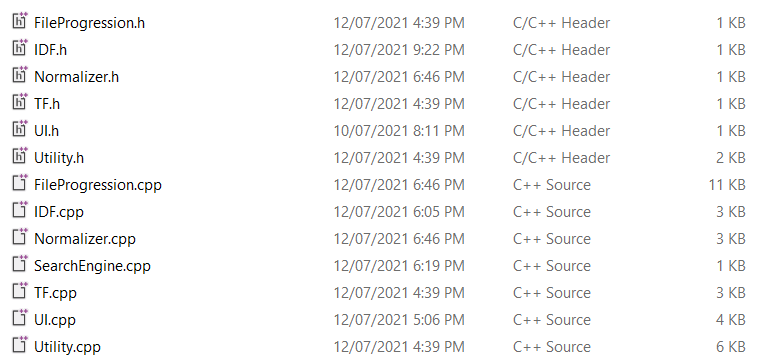
\includegraphics[scale=1]{Fig4}
\end{center}
\caption{Tổ chức các files mã nguồn trong chương trình}
\label{codefile}
\end{figure}
\subsection{Các files header}
\begin{itemize}
\item File header \textit{FileProgession.h} chứa các hàm tham gia vào việc xử lí các files dữ liệu đầu vào.
\item Các files header \textit{IDF.h}, \textit{TF.h} chứa các hàm tham gia vào việc tạo tập tin siêu dữ liệu (sẽ được nhắc đến trong phần sau).
\item File header \textit{Normalizer.h} giúp cho việc đơn giản hóa các kí tự tiếng Việt.
\item File header \textit{UI.h} chứa những hàm tạo nên giao diện người dùng trên console.
\item File header \textit{Utility.h} chứa các hàm bổ trợ khác.
\end{itemize}
\subsection{Các files source}
\begin{itemize}
\item Các file source có tên tương ứng với các files header thì chứa mô tả về các hàm trong file header đó.
\item File \textit{SearchEngine.cpp} chứa hàm main(), hàm chính của chương trình.
\end{itemize}
\newpage
\section{Các tập tin siêu dữ liệu (metadata)}
\subsection{TF và IDF}
TF \(-\) IDF là một kĩ thuật được sử dụng trong khai phá và truy hồi thông tin trong văn bản. Trọng số này được dùng để đánh giá tầm quan trọng của một từ trong một văn bản. Giá trị cao thể hiện độ quan trọng càng cao, phụ thuộc vào số lần xuất hiện của một từ trong một văn bản và số văn bản mà từ đó xuất hiện trong tập dữ liệu. Ngoài ra, TF và IDF còn được ứng dụng để loại bỏ những stopwords (những từ lặp lại nhiều nhưng không có ý nghĩa) trong các bài toán tóm tắt và phân loại văn bản. \cite{1}
\subsubsection{TF}
TF là viết tắt của từ tiếng Anh \textit{Term Frequency}, có nghĩa là tấn suất xuất hiện của từ trong văn bản. Vì các văn bản có thể có độ dài ngắn khác nhau nên một số từ có thể xuất hiện nhiều lần trong một văn bản dài hơn là một văn bản ngắn. Như vậy, giá trị của TF thường được tính bằng thương số của số lần xuất hiện và số lượng từ trong văn bản. \cite{1} \\
Trong phạm vi chương trình này, giá trị của TF (TF value) được tính như sau:
\begin{equation}
tf\left( {t,d} \right) = 0.5 + 0.5 \times \frac{{f\left( {t,d} \right)}}{{\max \left\{ {f\left( {w,d} \right):w \in d} \right\}}},
\label{tffor}
\end{equation}
trong đó
\begin{itemize}
\item \(tf\left( {t,d} \right)\) là giá trị TF của từ \(t\) trong văn bản \(d,\)
\item \({f\left( {t,d} \right)}\) là số lần xuất hiện của từ \(t\) trong văn bản \(d,\)
\item \({\max \left\{ {f\left( {w,d} \right):w \in d} \right\}}\) là số lần xuất hiện lớn nhất của một từ trong văn bản \(d.\)
\end{itemize}
Trong chương trình, TF được biểu diễn bằng các cấu trúc như sau:
\begin{lstlisting}
struct TF {
    string word;
    int count;
};

struct TF_list {
	int size;
	int capacity;
	int maxCount;
	TF* arrNorm;
};
\end{lstlisting}
Cấu trúc \lstinline{TF} được dùng để biểu diễn cho \textbf{một từ,} với \(2\) trường là \lstinline{word} và \lstinline{count}.
\begin{itemize}
\item Trường \lstinline{word} có kiểu \lstinline{string}, là từ mà ta đang xét,
\item Trường \lstinline{count} có kiểu \lstinline{int}, là số lần xuất hiện của từ đó trong văn bản.
\end{itemize}
Cấu trúc \lstinline{TF_list} được dùng để biểu diễn cho \textbf{một văn bản}, với \(4\) trường là \lstinline{size}, \lstinline{capacity}, \lstinline{maxCount}, \lstinline{arrNorm}.
\begin{itemize}
\item Trường \lstinline{size} có kiểu \lstinline{int}, là số lượng \lstinline{TF} có trong văn bản,
\item Trường \lstinline{capacity} có kiểu \lstinline{int}, là số lượng \lstinline{TF} tối đa có thể chứa, được khởi tạo và thay đổi phù hợp cho việc cấp phát động \lstinline{arrNorm},
\item Trường \lstinline{maxCount} có kiểu \lstinline{int}, là số lượng tối đa của \textbf{một từ} trong văn bản đó,
\item Trường \lstinline{arrNorm} là một mảng động để chứa các \lstinline{TF} trong văn bản.
\end{itemize}
Các hàm thao tác cho việc xử lí cấu trúc  \lstinline{TF} được viết trong file header \textit{TF.h} như sau:
\begin{figure}[H]
\begin{center}
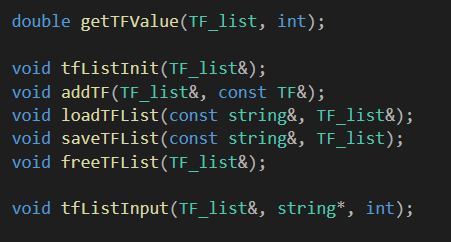
\includegraphics[scale=1]{Fig5}
\end{center}
\caption{Các hàm xử lí cấu trúc \lstinline{TF}}
\label{tffunc}
\end{figure}
\begin{itemize}
\item Hàm \lstinline{double getTFValue(const TF_list List, const int i)} được dùng để tính giá trị TF của phần tử thứ \lstinline{i} trong \lstinline{list} theo công thức (\ref{tffor}),
\item Hàm \lstinline{void TFListInit(TF_list& list)} khởi tạo một \lstinline{TF_list} mới,
\item Hàm \lstinline{void addTF(TF_list &List, const TF& Data)} có tác dụng thêm \lstinline{TF} \lstinline{Data} vào \lstinline{list},
\item Hàm \lstinline{void loadTFList(const string& Filename, TF_list& List)} được sử dụng để load các cấu trúc \lstinline{TF} từ tập tin có tên \lstinline{fileName} vào \lstinline{List},
\item Hàm \lstinline{void saveTFList(const string& Filename, const TF_list List)} dùng để lưu các giá trị từ \lstinline{List} vào tập tin có tên là \lstinline{fileName},
\item Hàm \lstinline{void FreeTFList(TF_list &List)} có tác dụng trả các vùng nhớ được cấp phát động sau khi sử dụng, tránh trình trạng memory leak,
\item Hàm \lstinline{void tfListInput(TF_list& List, string* Data, const int N)} có tác dụng tạo một \lstinline{TF_list} có kích thước là \lstinline{N} từ một mảng các \lstinline{string} đã được sắp xếp tăng dần là \lstinline{Data}.
\end{itemize}
\subsubsection{IDF}
IDF là viết tắt của từ tiếng Anh \textit{Inverse Document Frequency}, tạm dịch là nghịch đảo tần suất của văn bản, giúp đánh giá tầm quan trọng của một từ. Khi ta tính  toán TF, tất cả các từ được coi là có độ quan trọng như nhau. Nhưng một số stopwords như "is", "of", "that" trong tiếng Anh hay "à", "là", "đó", ... trong tiếng Việt thường xuất hiện rất nhiều lần nhưng độ quan trọng không cao. Như thế, chúng ta cần giảm độ quan trọng của những từ này xuống. \cite{1}\\
Trong phạm vi chương trình này, giá trị của IDF (IDF value) được tính như sau:
\begin{equation}
idf\left( {t,D} \right) = \log \frac{{{n_D}}}{{{n_d}:d \in D \wedge t \in d}},
\label{idffor}
\end{equation}
trong đó
\begin{itemize}
\item \(idf\left( {t,D} \right)\) là giá trị IDF của từ \(t\) trong thư mục \(D,\)
\item \({{n_D}}\) là tổng số văn bản trong thư mục \(D,\)
\item \({{n_d}:d \in D \wedge t \in d}\) là số văn bản nằm trong thư mục \(D\) và chứa từ \(t.\)
\end{itemize}
Logarithm cơ số \(10\) trong công thức không làm thay đổi tính tăng giảm của giá trị IDF của từ mà chỉ thu hẹp phạm vi giá trị của IDF. Việc sử dụng IDF nhằm giúp giá trị TF-IDF của một từ nhỏ hơn, vì chương trình sử dụng công thức tính giá trị TF-IDF của một từ trong một văn bản như sau:
\begin{equation}
tfidf\left( {t,d,D} \right) = tf\left( {t,d} \right) \times idf\left( {t,D} \right),
\label{tfidffor}
\end{equation}
trong đó
\begin{itemize}
\item \(tf\left( {t,d} \right)\) là giá trị TF của từ \(t\) trong văn bản \(d,\)
\item \(idf\left( {t,D} \right)\) là giá trị IDF của từ \(t\) trong thư mục \(D.\)
\end{itemize}
Từ đó, ta có thể thấy rằng những từ có giá trị TF-IDF cao là những từ xuất hiện nhiều ở một văn bản nhưng xuất hiện ít hoặc không xuất hiện ở các văn bản khác. Việc này giúp ta lọc ra những từ phổ biến và giữ lại những từ có giá trị cao, tạo thành tập các từ khóa của văn bản. \cite{1}\\
Tương tự như TF, trong chương trình, IDF được biểu diễn bằng các cấu trúc như sau:
\begin{lstlisting}
struct IDF {
	string word;
	int value;
};

struct IDF_list {
	int size;
	int capacity;
	int numFile;
	IDF* arrNorm;
};
\end{lstlisting}
Cấu trúc \lstinline{IDF} được dùng để biểu diễn \textbf{một từ}, với \(2\) trường là \lstinline{word} và \lstinline{value}.
\begin{itemize}
\item Trường \lstinline{word} có kiểu \lstinline{string}, là từ mà ta đang xét,
\item Trường \lstinline{value} có kiểu \lstinline{int}, là số lượng văn bản trong thư mục chứa từ đó.
\end{itemize}
Cấu trúc \lstinline{IDF_list} được dùng để biểu diễn cho \textbf{một thư mục}, với \(4\) trường là \lstinline{size}, \lstinline{capacity}, \lstinline{numFile} và \lstinline{arrNorm}.
\begin{itemize}
\item Trường \lstinline{size} có kiểu \lstinline{int}, là số lượng IDF có trong thư mục,
\item Trường \lstinline{capacity} có kiểu \lstinline{int}, là số lượng \lstinline{IDF} tối đa có thể chứa, được khởi tạo và thay đổi phù hợp cho việc cấp phát động \lstinline{arrNorm},
\item Trường \lstinline{numFile} có kiểu \lstinline{int}, là số lượng tập văn bản có trong thư mục,
\item Trường \lstinline{arrNorm} là một mảng động để chứa các \lstinline{IDF} trong thư mục.
\end{itemize}
Các hàm thao tác cho việc xử lí cấu trúc  \lstinline{IDF} được viết trong file header \textit{IDF.h} như sau:
\begin{figure}[H]
\begin{center}
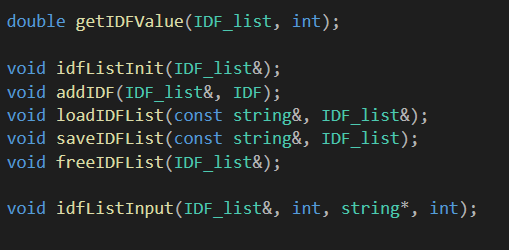
\includegraphics[scale=1]{Fig6}
\end{center}
\caption{Các hàm xử lí cấu trúc \lstinline{IDF}}
\label{idffunc}
\end{figure}
\begin{itemize}
\item Hàm \lstinline{double getIDFValue(const IDF_list List, const int i)} được dùng để tính giá trị IDF của phần tử thứ \lstinline{i} trong \lstinline{list} theo công thức (\ref{idffor}),
\item Hàm \lstinline{void idfListInit(IDF_list &List)} khởi tạo một \lstinline{IDF_list} mới,
\item Hàm \lstinline{void addIDF(IDF_list &List, IDF Data)} có tác dụng thêm \lstinline{IDF} \lstinline{Data} vào \lstinline{list},
\item Hàm \lstinline{void loadIDFList(const string& Filename, IDF_list &List)} được sử dụng để load các cấu trúc \lstinline{IDF} từ tập tin có tên \lstinline{fileName} vào \lstinline{List},
\item Hàm \lstinline{void saveIDFList(const string& Filename, const IDF_list List)} dùng để ghi các giá trị từ \lstinline{List} vào tập tin có tên là \lstinline{fileName},
\item Hàm \lstinline{void freeIDFList(IDF_list &List)} có tác dụng trả các vùng nhớ được cấp phát động sau khi sử dụng, tránh tình trạng memory leak,
\item Hàm \lstinline{void idfListInput(IDF_list& List, const int NumFile, string* Data, const int N)} có tác dụng tạo một \lstinline{IDF_list} cho một thư mục có \lstinline{NumFile} tập tin từ một mảng động các \lstinline{string} đã được sắp xếp tăng dần là \lstinline{Data}.
\end{itemize}
\subsection{Tạo các tập tin siêu dữ liệu}
\subsubsection{Yêu cầu cần tạo các tập tin siêu dữ liệu}
Nếu tìm kiếm những từ khóa đầu vào một cách bình thường, tuàn tự bằng cách duyệt từng văn bản thì sẽ tốn rất nhiều thời gian cho mỗi lần tìm kiếm, dẫn đến thời gian phản hồi kết quả lâu.\\
Do đó, ta cần phải rút trích các nội dung chính của từng văn bản, của từng thư mục để tạo ra các tập tin siêu dữ liệu rồi tìm kiếm trên các tập tin ấy.
\subsubsection{Tạo các tập tin siêu dữ liệu}
Hai header  files \textit{FileProgression.h} và \textit{Utility.h} chứa các hàm giúp cho việc tạo và sử dụng các tập tin siêu dữ liệu.
\begin{figure}[H]
\begin{center}
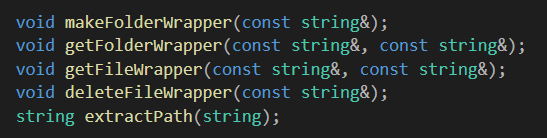
\includegraphics[scale=1]{Fig7}
\end{center}
\caption{Các hàm hỗ trợ tạo tập tin siêu dữ liệu trong \textit{Utility.h}}
\label{Fig7}
\end{figure}
\begin{figure}[H]
\begin{center}
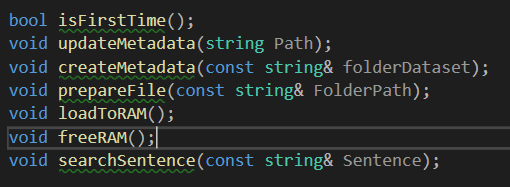
\includegraphics[scale=1]{Fig8}
\end{center}
\caption{Các hàm hỗ trợ tạo tập tin siêu dữ liệu trong \textit{FileProgression.h}}
\label{Fig8}
\end{figure}
Quy trình tạo các tập tin siêu dữ liệu như sau:
\begin{itemize}
\item Trước tiên, ta dùng lệnh \lstinline{dir} của \textit{Windows} để lấy tên của các thư mục con trong thư mục chứa dữ liệu cần tìm (dataset folder), lưu vào tập tin \textit{FolderList.txt},
\item Sau đó, ta tiếp tục dùng lệnh \lstinline{dir} để lấy tên của từng tập tin trong các thư mục con, tên các tập tin của thư mục A được lưu vào tập tin \textit{A.txt}, 
\item Tạo tập tin \textit{index.txt} chứa đường dẫn tương đối từ chương trình đến từng tập tin văn bản,
\item Ta chuyển các kí tự tiếng Việt từ dữ liệu đầu vào thành các kí tự Latin đơn giản bằng hàm \lstinline{std::string VEconvert(const std::wstring& Source)} trong header \textit{Normalize.h},
\item Tiếp theo đó, đối với từng tập tin văn bản trong cấc thư mục con, ta tạo các tập tin TF có tên tương ứng với tên của tập tin văn bản, ví dụ tập tin văn bản \textit{A.txt} thì tập tin TF tương ứng sẽ có tên là \textit{A.txt.tf},
\item Sau khi tạo xong các tập tin TF ứng với từng thư mục con, ta tạo tập tin IDF tương ứng với thư mục con đó, thư mục \textit{A} tương ứng với tập tin IDF là \textit{A.idf},
\item Sau đó, ta lặp lạp quá trình này cho các thư mục con khác của dataset folder.
\end{itemize}
Sau khi tạo xong các tập tin siêu dữ liệu, ta sẽ thu được các kết quả như sau:
\begin{itemize}
\item Tập tin \textit{FolderList.txt} lưu trữ nên các thư mục con trong dataset folder, cùng với tên của dataset folder ở dòng cuối cùng.
\begin{figure}[H]
\begin{center}
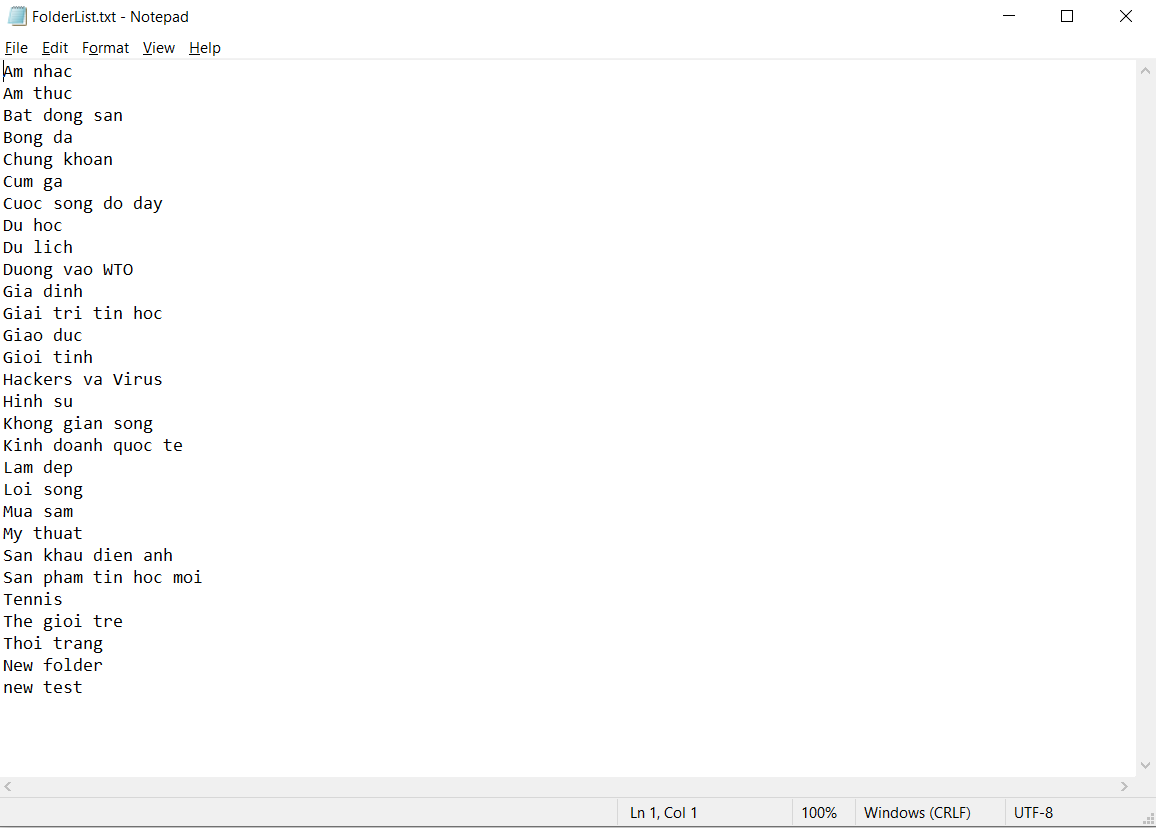
\includegraphics[scale=0.5]{Fig9}
\end{center}
\caption{Một ví dụ về tập tin \textit{FolderList.txt}}
\label{Fig9}
\end{figure}
\item Thư mục metadata chứa các tập tin siêu dữ liệu sẽ có các thư mục cùng tên với các thư mục con trong dataset folder, các tập tin văn bản chứa tên của từng tập tin trong các thư mục con, và các tập tin IDF tương ứng với các thư mục.
\begin{figure}[H]
\begin{center}
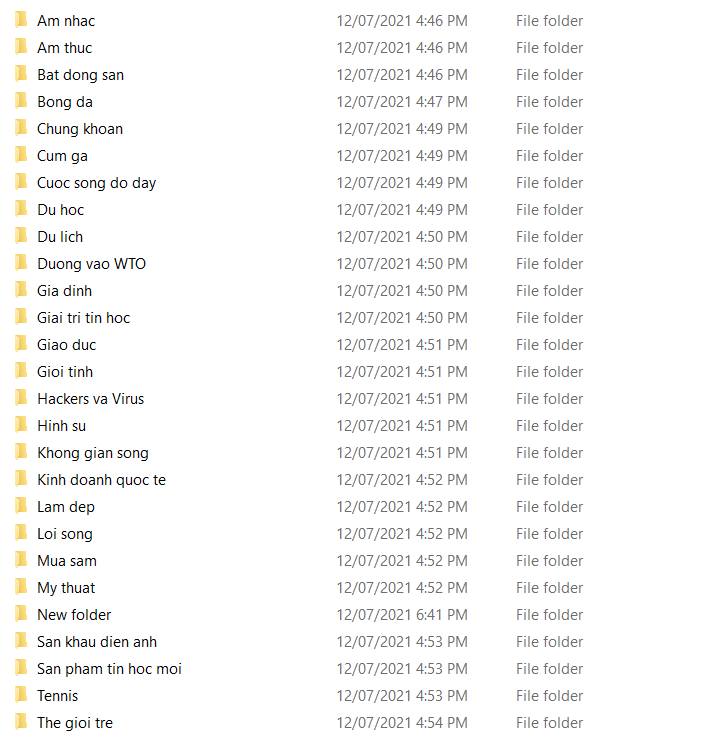
\includegraphics[scale=0.5]{Fig10}
\end{center}
\caption{Một ví dụ về các thư mục con trong thư mục \textit{metadata}}
\label{Fig10}
\end{figure}
\begin{figure}[H]
\begin{center}
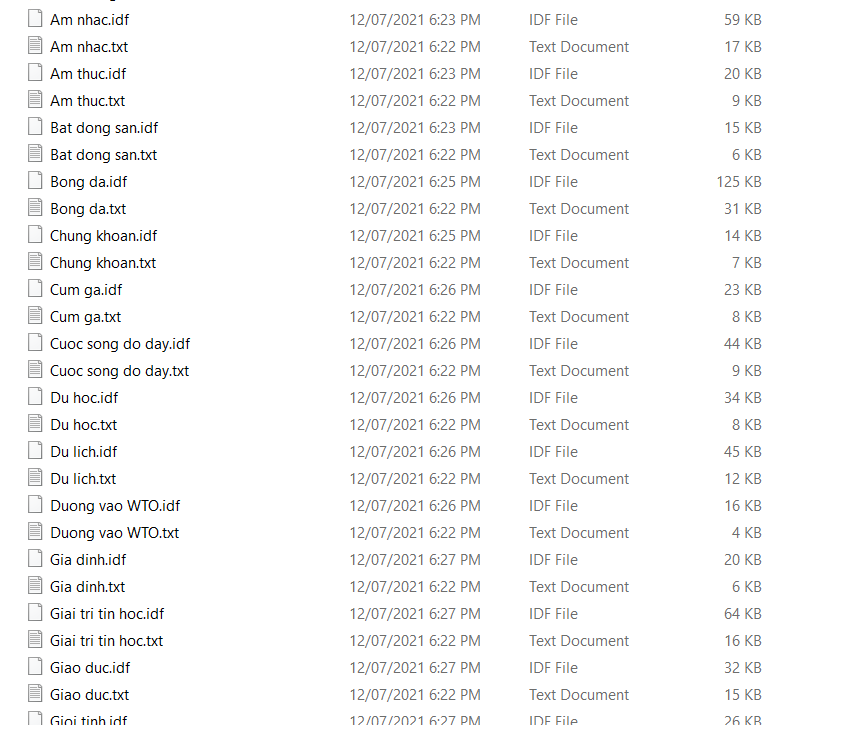
\includegraphics[scale=0.5]{Fig11}
\end{center}
\caption{Một ví dụ về các tập tin văn bản và tập tin IDF trong thư mục \textit{metadata}}
\label{Fig11}
\end{figure}
\item Trong từng thư mục con của thư mục \textit{metadata} sẽ chứa các tập tin TF tương ứng với các tập tin văn bản trong dataset folder.
\begin{figure}[H]
\begin{center}
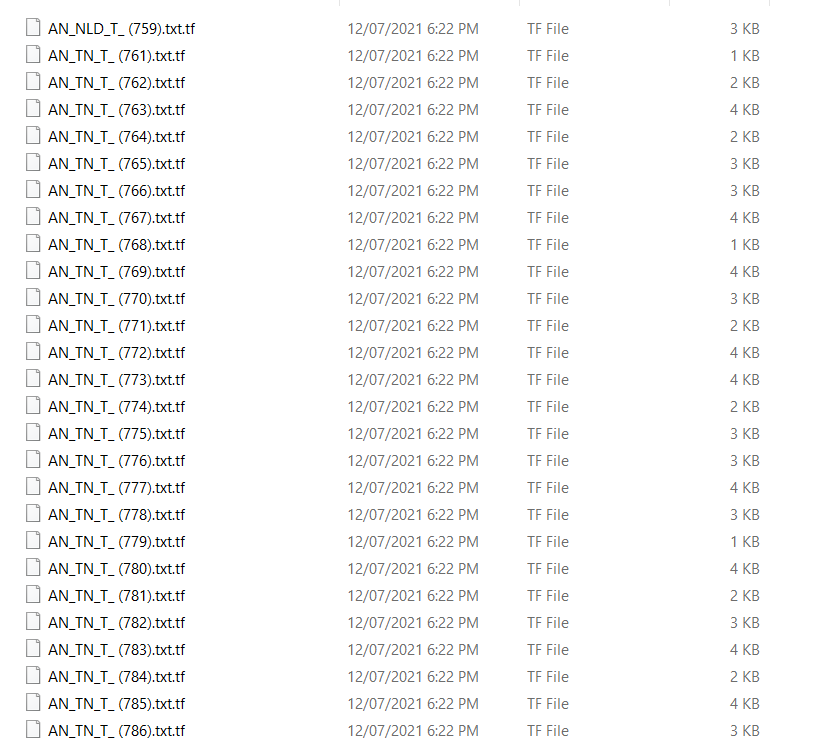
\includegraphics[scale=0.5]{Fig12}
\end{center}
\caption{Một ví dụ về thư mục con của \textit{metadata}}
\label{Fig12}
\end{figure}
\end{itemize}
\textbf{\textit{Lưu ý: Trong quá trình xử lí việc tạo/chỉnh sửa các tập tin siêu dữ liệu, chương trình sẽ tạo ra các tập tin và các thư mục như trên. Ta KHÔNG nên xóa hay có bất kì thao tác chỉnh sửa nào đối với các tập tin và thư mục này vì có thể dẫn đến việc chương trình cho ra kết quả sai hoặc gây ra lỗi trong việc vận hành của chương trình.}}
\newpage
\section{Xử lí dữ liệu tìm kiếm đầu vào}
Chương trình chạy trên console nên chỉ hỗ trợ tìm kiếm các từ không dấu. Chức năng tìm kiếm với các từ tiếng Việt có dấu chưa được hỗ trợ.\\
Sau khi người dùng nhập dữ liệu đầu vào, các từ sẽ được tách ra thành các tokens bằng  \lstinline{stringstream} trong thư viện \lstinline{sstream}. Sau đó, các tokens này được bỏ bớt các "punctuations" bằng hàm \lstinline{ispunct} của thư viện \lstinline{cctype}. Danh sách các punctuations được liệt kê trong hình \ref{punc} sau. \cite{3}
\begin{figure}[H]
\begin{center}

\includegraphics[scale=1]{Fig13}
\end{center}
\caption{Các "punctuations" trong C++}
\label{punc}
\end{figure}
Các tokens này được hàm \lstinline{void searchSentence(const string& Sentence)} trong \textit{FileProgression.h} xử lí, duyệt qua các \lstinline{IDF_list} của các thư mục, tìm kiếm xem có token đó hay không, nếu có thì ta tìm tiếp trong các \lstinline{TF_list} của các tập tin văn bản trong thư mục đó, nếu không thì ta bỏ qua thư mục đó, cứ như vậy đến hết các thư mục.\\
Do việc tìm kiếm tuần tự có thể tốn thời gian rất lâu, dựa vào việc khi tạo các tập tin siêu dữ liệu thì các từ đã được sắp xếp tăng dần, các thao tác tìm kiếm trong chương trình đều sử dụng thuật toán tìm kiếm nhị phân để có kết quả nhanh chóng.\\
Sau khi tìm được tất cả các tập tin chứa ít nhất một token, chương trình sẽ trả ra kết quả là tất cả các tập tin đó, với độ ưu tiên từ cao đến thấp, đi kèm là các tùy chọn cho người dùng (sẽ được nhắc đến trong phấn sau).\\
Mức độ ưu tiên của các tập tin được tính như sau:
\begin{itemize}
\item Tập tin nào có số tokens trùng khớp nhiều hơn được ưu tiên trước.
\item Nếu \(2\) tập tin có số tokens trùng khớp như nhau, tập tin có giá trị \(tfidf\left( {t,d,D} \right)\) cao hơn được ưu tiên trước.
\end{itemize}
Các cấu trúc mà chương trình sử dụng trong quá trình này:
\begin{itemize}
\item Cấu trúc \lstinline{FileData} dùng để quản lí các tập tin, gồm có \(4\) trường: \lstinline{posFolder}, \lstinline{posFile}, \lstinline{value} và \lstinline{intersectionCount}. 
\begin{lstlisting}
struct FileData {
	int posFolder;
	int posFile;
	double value;
	int intersectionCount;
};
\end{lstlisting}
\begin{itemize}
\item Trường \lstinline{posFolder} có kiểu \lstinline{int}, trường \lstinline{posFile} có kiểu \lstinline{int} tương ứng với vị trí của thư mục con trong danh sách thư mục và vị trí của tập tin trong danh sách tập tin của thư mục con đó. Danh sách thư mục được quản lí bởi một mảng động \lstinline{string* folder_list}, phần tử thứ \lstinline{i} của \lstinline{folder_list} là thư mục thứ \lstinline{i} trong danh sách thư mục con; danh sách tập tin trong thư mục con được quản lí bởi một mảng động hai chiều \lstinline{string** file_list}, phần tử \lstinline{file_list[i][j]} là tập tin thứ \lstinline{j} của thư mục con thứ \lstinline{i} trong danh sách,
\item Trường \lstinline{value} có kiểu \lstinline{doule} là giá trị \(tfidf\left( {t,d,D} \right)\) của token đang tìm trong tập tin đó,
\item Trường \lstinline{intersectionCount} có kiểu \lstinline{int} là số lượng tokens mà ta đang tìm trong tập tin. 
\end{itemize}
\item Cấu trúc \lstinline{FolderData} dùng để quản lí các thư mục, gồm có \(2\) trường: \lstinline{idfL} và \lstinline{tfLArr}.
\begin{lstlisting}
struct FolderData {
	IDF_list idfL;
	TF_list* tfLArr;
};
\end{lstlisting}
\begin{itemize}
\item Trường \lstinline{idfL} là \lstinline{IDF_list} tương ứng với thư mục,
 \item Trường \lstinline{tfLArr} là một mảng động các \lstinline{TF_list} tương ứng với thư mục này.
\end{itemize}
\item Cấu trúc \lstinline{ResponseData} là dữ liệu về kết quả phản hồi cho người dùng, gồm \(3\) trường: \lstinline{file}, \lstinline{size} và \lstinline{cap}.
\begin{lstlisting}
struct ResponseData {
	FileData* file;
	int size;
	int cap;
};
\end{lstlisting}
\begin{itemize}
\item Trường \lstinline{file} là một mảng động các \lstinline{fileData}, chứa danh sách các tập tin có chứa các tokens đang tìm,
\item Trường \lstinline{size} là số lượng các phần tử của \lstinline{file},
\item Trường \lstinline{cap} là số lượng tối đa các phần tử mà \lstinline{file} có thể chứa, được khởi tạo và thay đổi cho phù hợp.
\end{itemize}
\item Ngoài ra còn sử dụng một vài cấu trúc phụ khác.
\end{itemize}
\newpage
\section{Quá trình hoạt động của chương trình}
\subsection{Lần chạy đầu tiên}
Khi khởi động, chương trình sẽ kiểm tra xem đây có phải là lần chạy đầu tiên hay không (do lần đầu tiên chưa có các tập tin siêu dữ liệu). Nếu có, chương trình sẽ yêu cầu người dùng nhập tên của dataset folder như hình dưới. Ở đây, dataset folder được nhập vào có tên là \textit{new train}.
\begin{figure}[H]
\begin{center}
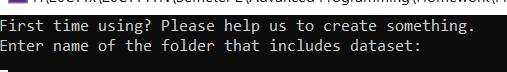
\includegraphics[scale=1]{Fig14}
\label{Fig14}
\end{center}
\caption{Nhập tên của dataset folder ở lần chạy đầu tiên}
\end{figure}
Sau khi nhập tên của dataset folder xong, chương trình sẽ tiến hành tạo các tập tin siêu dữ liệu theo quy trình bên trên. Quá trình này có thể tốn một vài phút, tùy vào số lượng tập tin văn bản trong thư mục dataset.
\begin{figure}[H]
\begin{center}
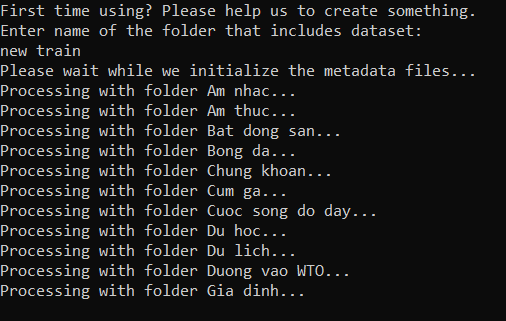
\includegraphics[scale=1]{Fig15}
\end{center}
\caption{Chương trình đang tạo các tập tin siêu dữ liệu cho lần chạy đầu tiên}
\label{Fig15}
\end{figure}
\textbf{\textit{Lưu ý: các tập tin văn bản trong thư mục dataset cần phải ở dạng UTF-16, nếu không chương trình sẽ bị những lỗi không mong muốn.}}
\begin{figure}[H]
\begin{center}
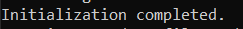
\includegraphics[scale=2]{Fig16}
\end{center}
\caption{Thông báo tạo thành công các tập tin siêu dữ liệu}
\label{Fig16}
\end{figure}
\subsection{Load dữ liệu vào RAM}
Sau khi tạo xong các tập tin siêu dữ liệu ở lần gọi đầu tiên, hoặc khi ta khởi động chương trình các lần tiếp theo, chương trình sẽ tiến hành load dữ liệu từ database về các tập tin siêu dữ liệu vào RAM.
\begin{figure}[H]
\begin{center}
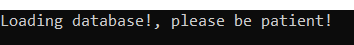
\includegraphics[scale=2]{Fig17}
\end{center}
\caption{Chương trình đang tiến hành load dữ liệu từ database}
\label{Fig17}
\end{figure}
\subsection{Menu của chương trình}
Sau khi dữ liệu được đưa vào RAM, chương trình sẽ hiển thị một menu bao gồm các tính năng mà chương trình hỗ trợ.
\begin{figure}[H]
\begin{center}
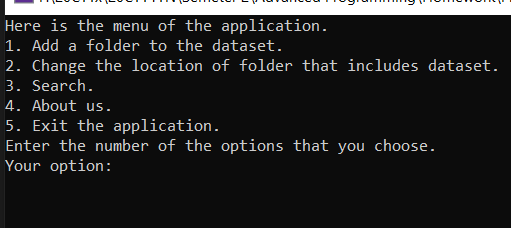
\includegraphics[scale=1]{Fig18}
\end{center}
\caption{Menu của chương trình}
\end{figure}
Ta có thể thấy các tính năng được liệt kê của chương trình bao gồm:
\begin{itemize}
\item Thêm một thư mục vào dataset folder,
\item Đổi sang một dataset folder khác,
\item Tìm kiếm
\item Thông tin về người phát triển của chương trình,
\item Thoát khỏi chương trình
\end{itemize}
\subsubsection{Thêm một thư mục vào dataset folder}
Khi ta chọn tùy chọn đầu tiên này, chương trình sẽ yêu cầu ta nhập đường dẫn đến thư mục cần thêm. Đường dẫn được nhập ở đây phải là \textbf{đường dẫn tuyệt đối} hoặc \textbf{tương đối với thư mục chứa chương trình}, ví dụ \textit{F:\(\backslash\)Folder Needs Adding}. Các tập tin trong thư mục này cũng phải có định dạng \textbf{UTF-16}, nếu không sẽ dẫn đến những lỗi không mong muốn cho chương trình.\\
Sau đó, thư mục này sẽ được thêm vào dataset folder, chương trình sẽ tạo các tập tin siêu dữ liệu tương ứng với thư mục này tương tự như với các thư mục khác. Tên của thư mục này được đưa vào \textbf{cuối} tập tin \textit{FolderList.txt}. Tiếp theo đó, chương trình sẽ tự động cập nhật database rồi load vào RAM.\\
Sau khi thêm thư mục thành công, chương trình sẽ báo như hình \ref{Fig19}. Ta có thể vào thư mục \textit{metadata} để kiểm tra thành quả.\\
\textbf{\textit{Lưu ý: chương trình chưa hỗ trợ việc thêm trực tiếp một tập tin văn bản vào dataset folder, do đó, ta cần phải đóng gói các tập tin văn bản vào một thư mục trước khi thêm.}}
\begin{figure}[H]
\begin{center}
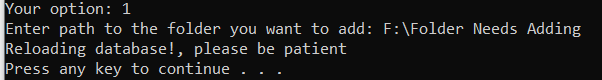
\includegraphics[scale=1]{Fig19}
\end{center}
\caption{Ví dụ thêm thư mục vào dataset folder}
\label{Fig19}
\end{figure}
\subsubsection{Đổi sang một dataset folder khác}
Đối với tùy chọn thứ 2 này, chương trình sẽ yêu cầu ta nhập tên của thư mục dataset folder mới. \\
Thư mục dataset mới cần phải nằm cùng thư mục với chương trình.\\
Sau khi nhận được tên của dataset folder mới, chương trình sẽ tiến hành giải phóng các tập tin siêu dữ liệu cũ, rồi lặp lại quy trình tạo các tập tin siêu dữ liệu đối với thư mục mới. Thời gian tiêu tốn của quá trình này phụ thuộc vào kích thước của thư mục dataset folder.\\
Sau khi thành công, chương trình sẽ thông báo như hình \ref{Fig20}.
\begin{figure}[H]
\begin{center}
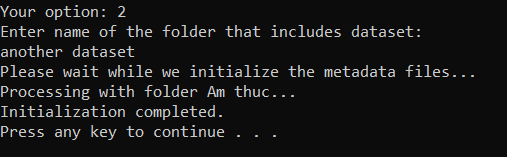
\includegraphics[scale=1]{Fig20}
\end{center}
\caption{Thay đổi dataset folder}
\label{Fig20}
\end{figure}
\subsubsection{Tìm kiếm}
Đây là phần mấu chốt, là mục tiêu của đồ án này. Việc tìm kiếm chỉ có thể thực hiện sau khi các tập tin siêu dữ liệu được tạo và dữ liệu được load vào RAM. Khi ta chọn tùy chọn này, chương trình sẽ yêu cầu ta nhập từ khóa (keyword) để tìm kiếm như hình \ref{Fig21}.
\begin{figure}[H]
\begin{center}
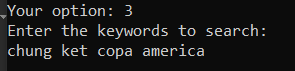
\includegraphics[scale=2]{Fig21}
\end{center}
\caption{Nhập từ khóa tìm kiếm}
\label{Fig21}
\end{figure}
Sau đó, chương trình sẽ tiến hành xử lí và trả kết quả như hình \ref{Fig22} sau.
\begin{figure}[H]
\begin{center}
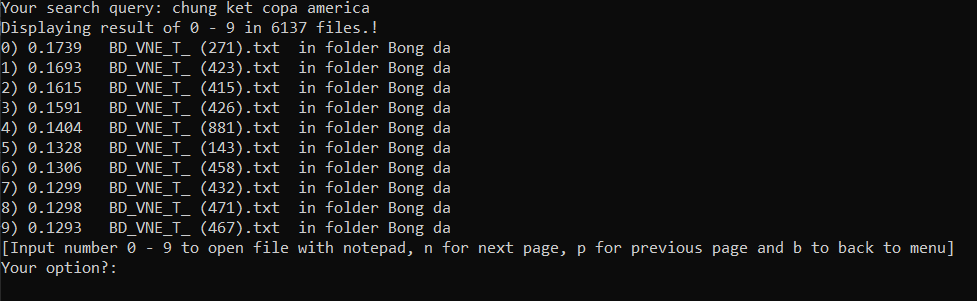
\includegraphics[scale=0.8]{Fig22}
\end{center}
\caption{Kết quả tìm kiếm}
\label{Fig22}
\end{figure}
Từ đó, ta có thể thấy các tính năng hỗ trợ người dùng trên giao diện kết quả như sau:
\begin{itemize}
\item Cho biết tổng số tập tin chứa ít nhất một \textbf{từ đơn} trong từ khóa cần tìm, cho biết ta đang xem các tập tin có thứ tự bao nhiêu.
\item Cho biết thư mục chứa tập tin đó, cũng như giá trị \(tfidf\left( {t,d,D} \right)\) của từ trong văn bản đó làm căn cứ để xếp hạng độ ưu tiên.
\item Tính năng giúp mở tập tin bất kì trong danh sách kết quả với Notepad như hình \ref{Fig23}.\\
\textbf{\textit{Lưu ý: sau khi mở và xem một tập tin với Notepad, để chương trình có thể tiếp tục hoạt động, ta cần đóng tập tin đó lại.}}
\begin{figure}[H]
\begin{center}
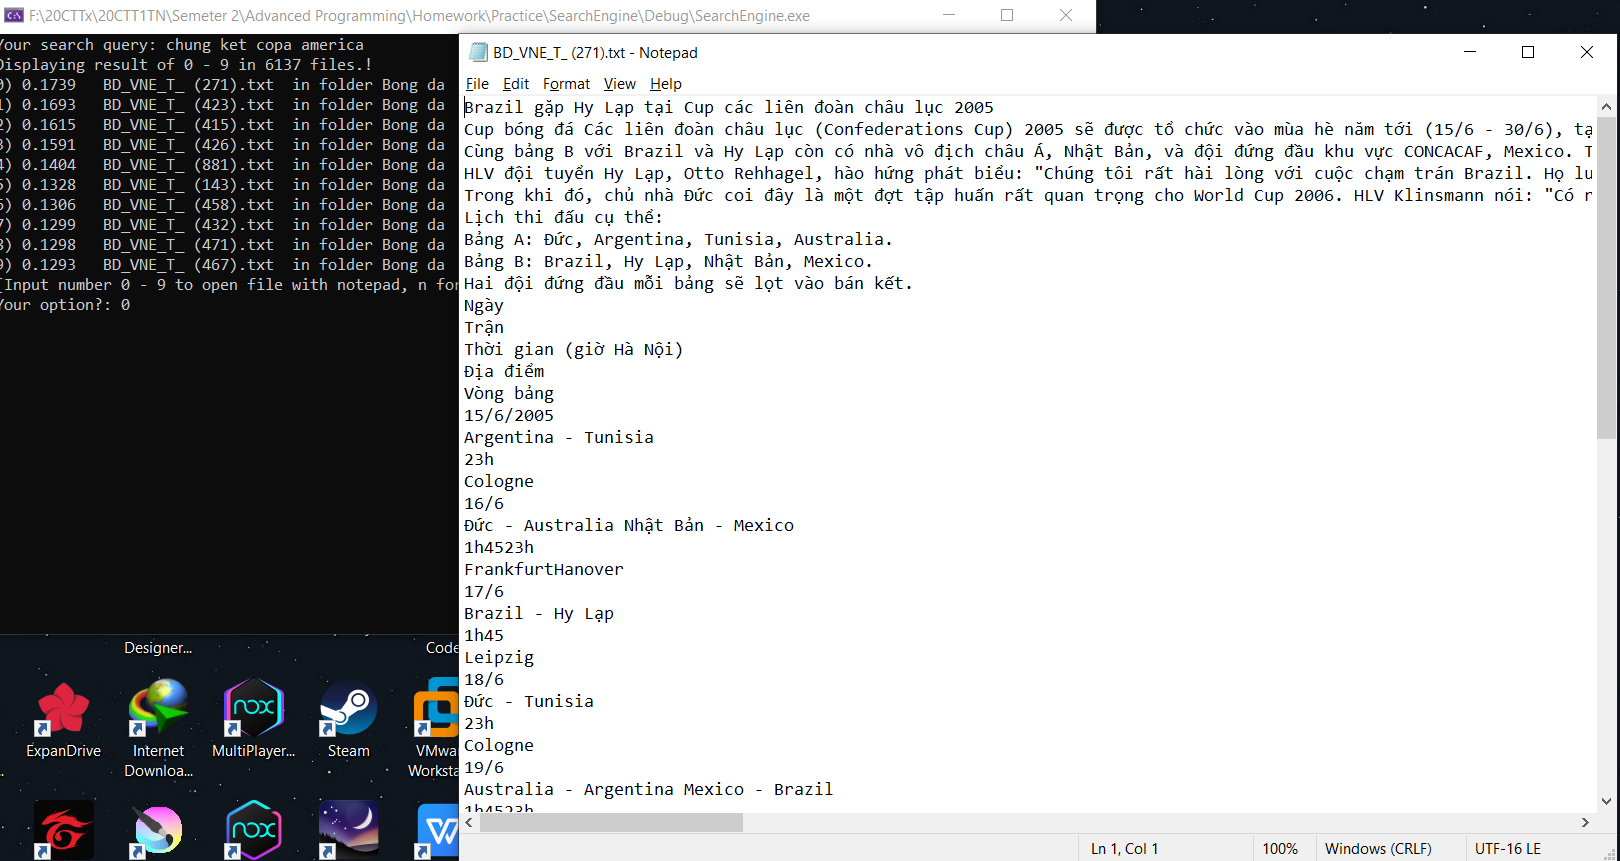
\includegraphics[scale=0.5]{Fig23}
\end{center}
\caption{Mở tập tin kết quả với Notepad}
\label{Fig23}
\end{figure}
\item Tính năng \textit{next page} (hình \ref{Fig24}) và \textit{previous page} (hình \ref{Fig25}) giúp ta đi đến trang trước hoặc trang sau của trang kết quả tìm kiếm hiện tại.
\begin{figure}[H]
\begin{center}
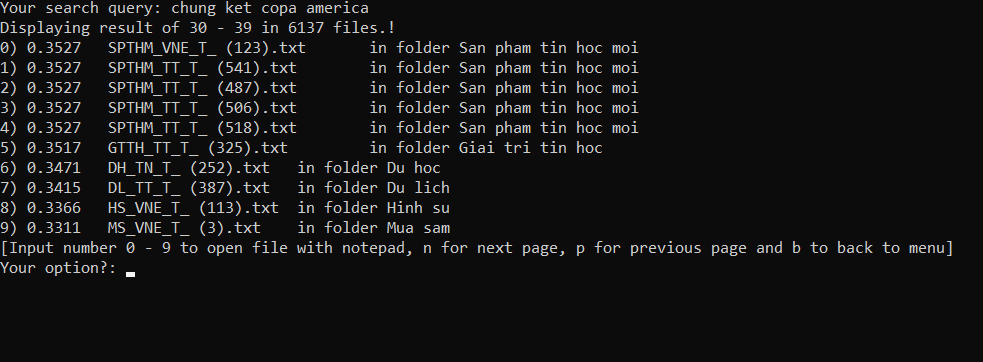
\includegraphics[scale=0.9]{Fig24}
\end{center}
\caption{Tính năng \textit{next page}}
\label{Fig24}
\end{figure}
\begin{figure}[H]
\begin{center}
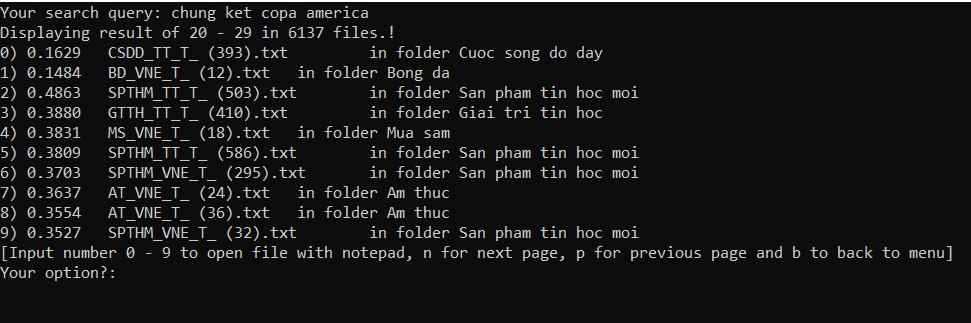
\includegraphics[scale=0.9]{Fig25}
\end{center}
\caption{Tính năng \textit{previous page}}
\label{Fig25}
\end{figure}
\item Tính năng \textit{back} giúp ta quay về menu chính của chương trình.
\end{itemize}
\subsubsection{Thông tin về người phát triển của chương trình}
Khi ta chọn tùy chọn này, màn hình sẽ hiển thị thông tin về các tác giả của chương trình như hình \ref{Fig26}.
\begin{figure}[H]
\begin{center}
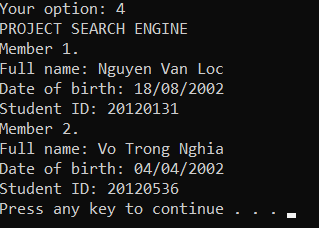
\includegraphics[scale=1]{Fig26}
\end{center}
\caption{About us}
\label{Fig26}
\end{figure}
\subsubsection{Thoát khỏi chương trình}
Đây là tùy chọn giúp ta thoát khỏi chương trình.
\begin{figure}[H]
\begin{center}
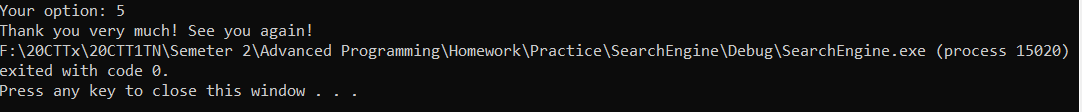
\includegraphics[scale=0.8]{Fig27}
\end{center}
\caption{Thoát khỏi chương trình}
\label{Fig27}
\end{figure}
\newpage
\section{Tài nguyên chương trình tiêu tốn}
\subsection{Cấu hình máy dùng để chạy thử chương trình}
Chương trình được chạy thử trên máy có cấu hình như trong hình \ref{Fig28}.
\begin{figure}[H]
\begin{center}
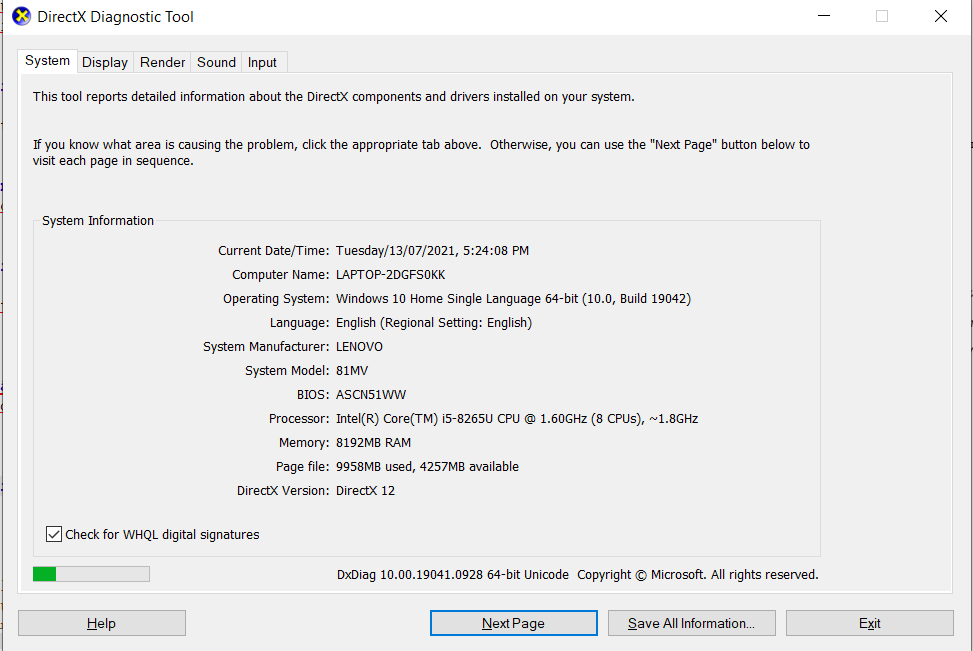
\includegraphics[scale=0.62]{Fig28}
\end{center}
\caption{Cấu hình máy chạy thử chương trình.}
\label{Fig28}
\end{figure}
\subsection{Thời gian chạy thử chương trình}
Ở đây ta sẽ chú trọng vào thời gian xử lí việc tạo tập tin siêu dữ liệu và thời gian xử lí việc load database vào RAM.\\
Thư mục dataset folder có \(14377\) tập tin văn bản với tổng kích thước là khoảng \(66.9\) MB như hình \ref{Fig29}.
\begin{figure}[H]
\begin{center}
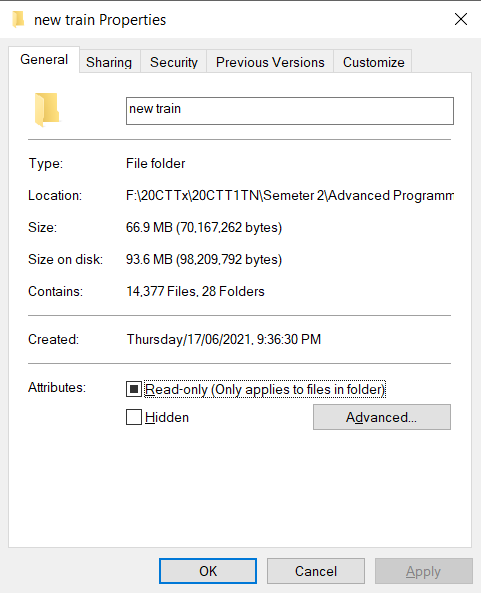
\includegraphics[scale=1]{Fig29}
\end{center}
\caption{Kích thước dataset folder}
\label{Fig29}
\end{figure}
Với tập dữ liệu trên, các thông số thời gian đo được là:
\begin{itemize}
\item Thời gian tạo các tập tin siêu dữ liệu là khoảng \(647.29\) giây.
\begin{figure}[H]
\begin{center}
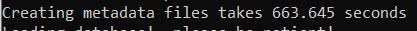
\includegraphics[scale=2]{Fig30}
\end{center}
\caption{Thời gian tạo các tập tin siêu dữ liệu}
\label{Fig30}
\end{figure}
\item Thời gian load database lên RAM khoảng \(12.704\) giây.
\begin{figure}[H]
\begin{center}
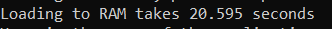
\includegraphics[scale=2]{Fig31}
\end{center}
\caption{Thời gian load dữ liệu vào RAM}
\label{Fig31}
\end{figure}
\end{itemize}
Thời gian tìm kiếm các từ khóa phụ thuộc vào độ dài và số lượng \textbf{từ đơn} của từ khóa, dao động khoảng \(1\) đến \(2\) giây.
\subsection{Bộ nhớ và CPU tiêu tốn}
\begin{itemize}
\item Trong quá trình tạo các tập tin siêu dữ liệu:
\begin{figure}[H]
\begin{center}
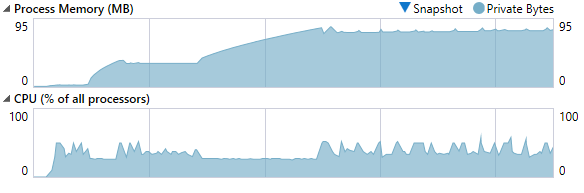
\includegraphics[scale=0.75]{Fig33}
\end{center}
\caption{Tài nguyên máy tính sử dụng khi tạo tập tin siêu dữ liệu}
\label{Fig33}
\end{figure}
\item Trong quá trình load dữ liệu từ database vào RAM:
\begin{figure}[H]
\begin{center}
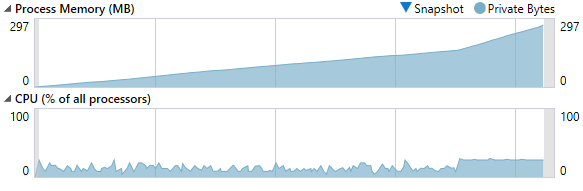
\includegraphics[scale=0.75]{Fig34}
\end{center}
\caption{Tài nguyên máy tính sử dụng khi load dữ liệu vào RAM}
\label{Fig34}
\end{figure}
\end{itemize}
\newpage
\section{Nhận xét về chương trình và dự án}
\subsection{Về thời gian chạy của từng quá trình}
\begin{itemize}
\item Hầu hết quá trình tạo/cập nhật các tập tin siêu dữ liệu là sắp xếp trên chuỗi bằng thuật toán merge sort. Merge sort đã được nhóm cải tiến sử dụng đa luồng, giúp sử dụng CPU hiệu quả hơn và giảm được gần một nửa thời gian chạy so với bình thường.
\item Trong quá trình load dữ liệu từ database vào RAM, chương trình sử dụng một khoảng thời gian bình thường, do không có các quá trình nào tiêu tốn quá nhiều thời gian.
\item Trong quá trình tìm kiếm và trả kết quả cho người dùng, do dữ liệu trong các tập tin TF và IDF đã được sắp xếp tăng dần nên thuật toán tìm kiếm nhị phân giúp xác định nhanh chóng \textit{tất cả} các kết quả cần tìm.
\end{itemize}
\subsection{Về bộ nhớ}
\begin{itemize}
\item Lớp \lstinline{std::string} trong thư viện chuẩn của C++ được sử dụng xuyên suốt cả chương trình, đảm bảo an toàn về mặt bộ nhớ và dữ liệu được lưu trong heap.
\item Một vài mảng động các \lstinline{string} được vận dụng khi cần thiết, giảm thiểu việc allocate và de-allocate liên tục, gây ảnh hưởng đến performance của chương trình.
\item Mỗi hàm sau khi kết thúc sẽ thực hiện trả vùng nhớ, đảm bảo tối ưu vùng nhớ heap.
\item Không gây ra tình trạng memory leak trong chương trình.
\end{itemize}
\subsection{Về cấu trúc chương trình}
\begin{itemize}
\item Các files được chia hợp lý, thể hiện được các mục đích nhất định và không quá phụ thuộc vào nhau.
\item Chương trình khi chạy luôn đảm bảo tham số đầu vào đúng mục đích.
\end{itemize}
\subsection{Về quản lý dự án}
Dự án được cooperated bởi hai thành viên trên nền tảng Github, đảm bảo tiến độ hoàn thành và quản lý các hàm, hỗ trợ sửa lỗi về sau.
\begin{figure}[H]
\begin{center}
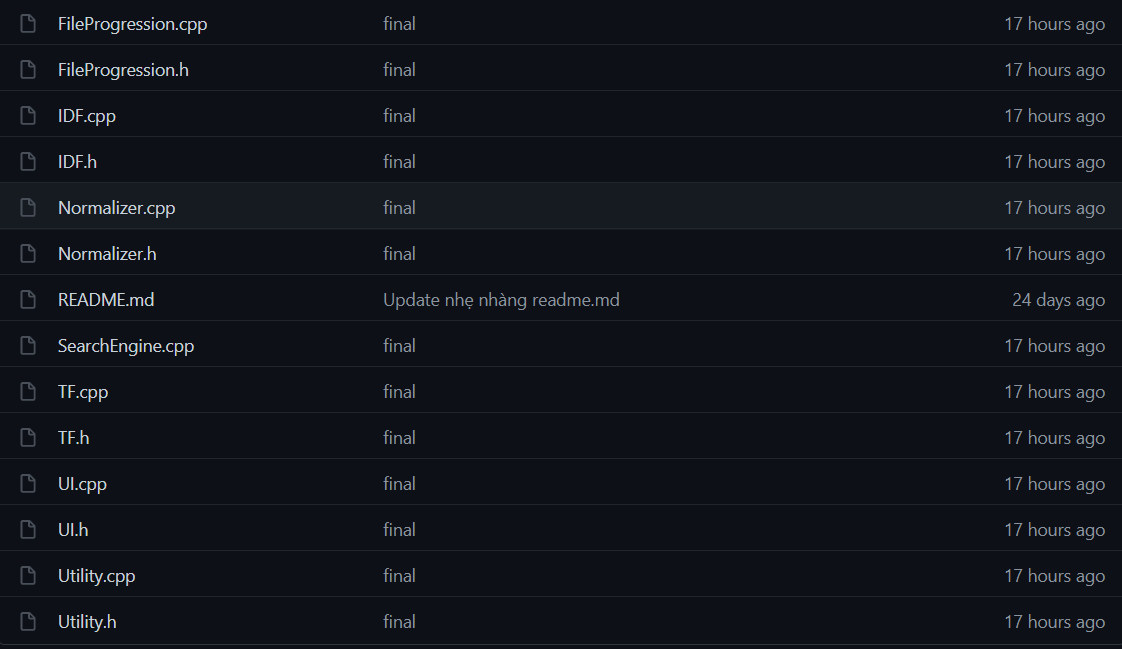
\includegraphics[scale=0.4]{Fig32}
\end{center}
\caption{Quản lí dự án bằng Github}
\label{Fig32}
\end{figure}
\newpage
\begin{thebibliography}{99}
\bibitem{1} \url{https://nguyenvanhieu.vn/tf-idf-la-gi/}
\bibitem{2} \url{https://vi.wikipedia.org/wiki/Tf%E2%80%93idf}
\bibitem{3} \url{https://www.programiz.com/c-programming/library-function/ctype.h/ispunct}
\bibitem{4} \url{https://www.geeksforgeeks.org/}
\bibitem{5} \url{https://stackoverflow.com/}
\bibitem{6} \url{https://www.cplusplus.com/}
\end{thebibliography}
\end{document}